\section*{Problem 1: Naive Bayes vs. Logistic Regression [Nicole - 30pts]}

Naive Bayes (NB) and Logistic Regression (LR) form what is called a \textit{generative-discriminative pair} of classifiers. In this problem, we will explore their relationship in some detail.

Assume that we are performing a binary classification task with $n$ samples. Each sample has $p$ binary features $X_1,\hdots,X_p \in \{0,1\}$, and a corresponding label $Y \in \{0,1\}$.
\begin{enumerate}
\item
    For each of Naive Bayes and Logistic Regression briefly state: 
	\begin{enumerate}
	\item 
	The formula for the conditional likelihood, $P(Y = 1\mid X_,\hdots,X_p)$, assumed by each model. 
	{\bf [4 pts]}
	\item 
	The classification rule.
	{\bf [2 pts]}
	\item 
	The parameters we have to estimate.
	{\bf [2 pts]}
	\item 
	The method we use to do Maximum Likelihood Estimation (MLE) of the parameters. 
	{\bf [2 pts]}
	\end{enumerate}
\item
Next, we show that Naive Bayes and Logistic Regression form a pair: 
	\begin{enumerate}
	\item 
	Briefly describe (in one sentence) what makes two classifiers a generative-discriminative pair. 
	{\bf [2 pt]}
	\item 
	Generative vs. discriminative algorithms learn parameters which have completely different intuitive interpretations. Figure \ref{fig:sampledata} is a plot of a sample data set with two features, $X_1, X_2 \in \mathbb{R}$. Draw on the plot a visualization of what the parameters encode for Naive Bayes and Logistic Regression respectively. Please clearly indicate which is which.
	{\bf [2 pts]}
	
		\begin{figure}[ht]
	\centering
	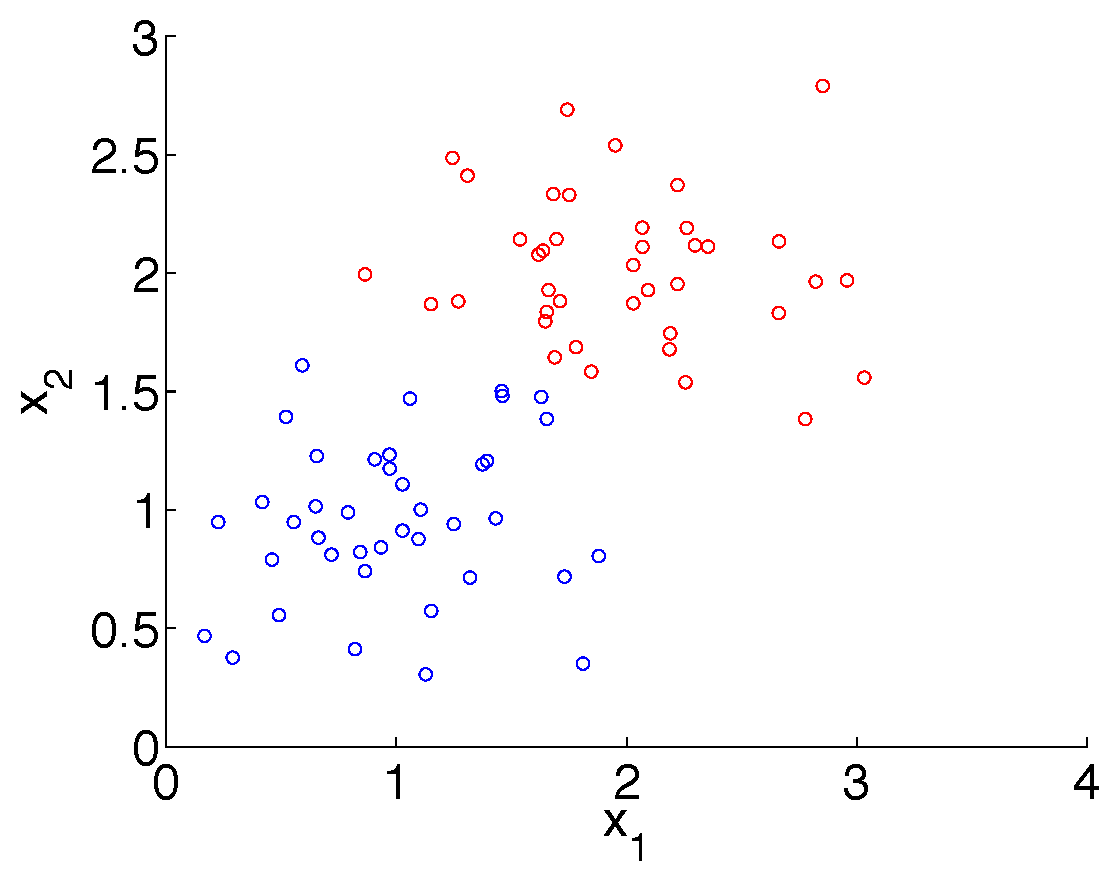
\includegraphics[width = 0.5\linewidth]{pics/gaussian_lr_nb.pdf}
	\caption{A sample data set. Clearly indicate with solid or dashed lines what the parameters learned in Naive Bayes and Logistic Regression respectively encode.}
	\label{fig:sampledata}
	\end{figure}

	\item 
	Prove that we can write the Naive Bayes class distribution $P(Y = 1\mid X_,\hdots,X_p)$ in a form that matches the Logistic class distribution. To start, it will help to write $P(X_j = 1\mid Y = 1) = \theta_{j}$. Hint: this makes $P(X_j = x\mid Y=1) = \theta_{j}^{x}(1 - \theta_{j})^{x}$.
	{\bf {\bf [4 pts]}}
	\item 
	Show that Logistic Regression is the discriminative version of Naive Bayes. Hint: what happens when you optimize the conditional likelihood you derived in the previous part? 
	{\bf {\bf [2 pts]}}
	\item 
	The classifier we learn by optimizing the Naive Bayes conditional likelihood is nevertheless not the same as what we would have learned had we learned a Logistic classifier directly. What modeling assumption makes it somewhat less generic than Logistic Regression?
	{\bf [2 pt]}
	\item 
	Under what circumstances would Naive Bayes and Logistic Regression produce (asymptotically) the same classifier?
	{\bf [2 pt]}
	\end{enumerate}
			\item
Let's compare the performance properties of these two algorithms. Let $h_l$ be a Logistic Regression classifier, and $h_b$ be a Naive Bayes classifier. Let $h_l^*$ be the best possible Logistic classifier, and $h_b^*$ the best possible Naive Bayes Classifier. These are the classifiers we would get if we had an infinite amount of data on which to train. The error rate of a classifier $h$ is given by $\epsilon(h)$.
	\begin{enumerate}
	\item 
	Which classifier ($h_l$ or $h_b$) will generally have a lower asymptotic error rate? Hint: think about what we showed in part 2 this question.
	{\bf [2 pts]}
	\item 
	Recall that we are performing classification in $p$ dimensions (i.e. with $p$ features) and have $n$ samples. The error rate for $h_l$ can be bounded as follows (note that we will be able to prove this later in the course; for now you can take it for granted):
	\[\epsilon(h_l) \leq \epsilon(h_l^*) + O\bigg(\sqrt{\frac{p}{n}\log\frac{p}{n}}\bigg)\]
	How many samples do we need (on what order should $n$ be) to keep $\epsilon(h_l) = O(\epsilon(h_l^*))$? 
	{\bf [1 pt]}
	\item 
	The parameters of $h_b$ are guaranteed to be within $O\bigg(\sqrt{\frac{1}{n}\log p}\bigg)$ of those of $h_b^*$. How many samples do we need to feel confident that the performance of $h_b$ is close to that of $h_b^*$?
	{\bf [1 pt]}
	\item 
	Given the answers to parts (b) and (c), can you think of a situation in which it would be better to use $h_b$ than $h_l$?
	{\bf [2 pts]} \\\\
	\end{enumerate}
\end{enumerate}
